\chapter{模擬データによる定量評価}
% 3.1 模擬データの生成方法
% 3.2 解析方法
%  3.2.1 ベイズ推定の基礎
%  3.2.2 解析に用いる尤度関数
% 3.3 模擬データを用いた定量評価の結果
%  3.3.1 asymmetric driftの影響 (今、メールでは名称を省略しています)
%  3.3.2 ...影響
%  3.3.7 ...影響
% 3.4 解析結果のまとめ


Gaiaの模擬データを生成し、それを解析することで、Asymmetri drift、視線速度の有無、速度楕円体の傾き、太陽からの距離$D$、円盤面からの距離$|z|$、データ数のそれぞれの解析への影響を定量的に評価した。この章ではそれらの結果についてまとめる。
\section{模擬データの生成方法}
観測方程式(\ref{ObsEq})に従う速度場を仮定し、密度分布には指数関数的密度分布$\rho(R,z) = \rho_0 e^{-R/R_d} e^{-z/z_d},R_d=3 \mathrm{kpc},z_d=300 \mathrm{pc}$(\cite{BH2016})を仮定している。ここで、$R,z$はそれぞれ円筒座標系での動径方向と鉛直方向の位置、$R_d,z_d$は$R,z$方向の密度分布のスケール長を示す。サンプル数は基本的に1000とし、太陽からの距離$D<1\,\mathrm{kpc}$としている。このときの3次元分布と1次元の頻度分布太陽の銀河中心からの距離は$R_0 = 8.2\ \mathrm{kpc}$(\cite{BH2016})としている。また、asymmetric driftは速度分散の銀河回転方向成分を用いて$v_{\mathrm{a}} = \sigma_R^2$として計算している。

%\subsection{模擬データの生成コード}
%以下に模擬データの作成コードのうちの1つを記述する。このコードではexponential diskを仮定し、太陽からの距離1kpc以内に1000個の星があるとしている。OLCODモデルに従った速度場を持たせている。
%\lstinputlisting[language=Python]{code/MockGenerate.py}

\begin{figure*}[htbp]
\begin{center}
	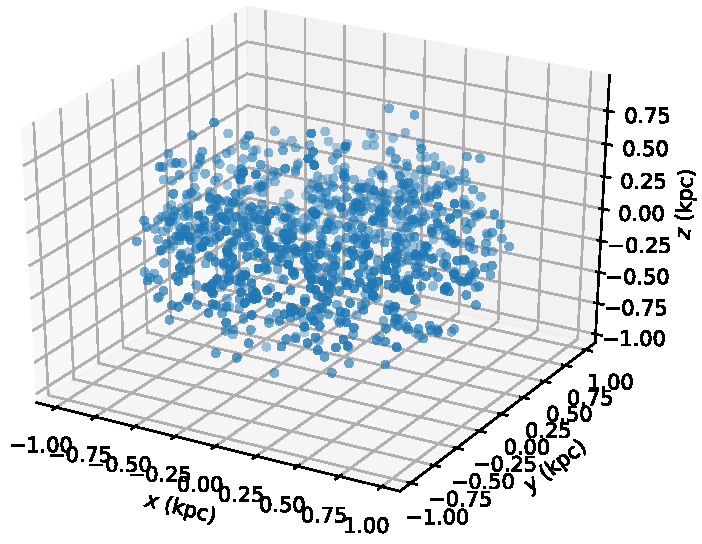
\includegraphics[width=9cm]{fig/3dMockData.pdf}
	\caption{1000個の星の模擬データの3次元分布} \label{dist3dMockData}
\end{center}
\end{figure*}

\begin{figure*}
   \centering
\begin{tabular}{ccc}
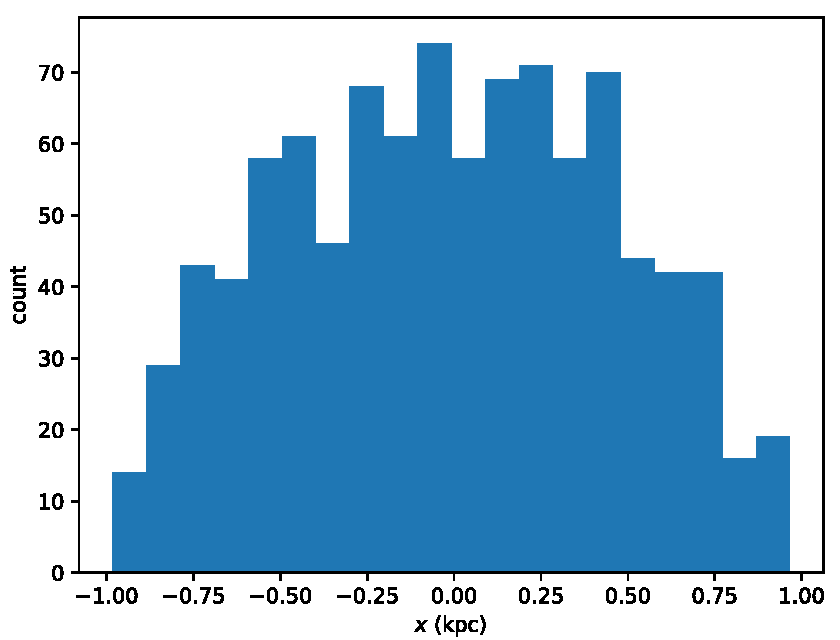
\includegraphics[width=4.5cm]{fig/dist_x.pdf}&
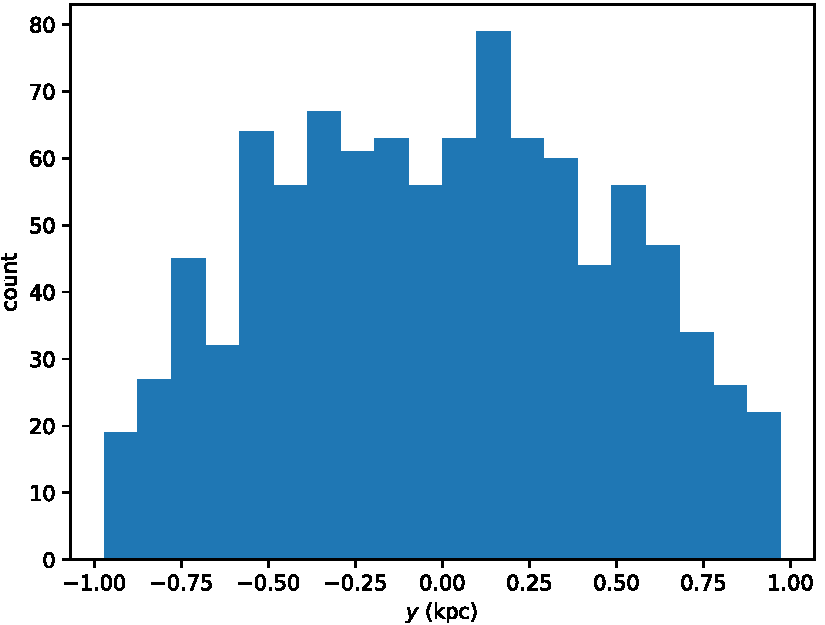
\includegraphics[width=4.5cm]{fig/dist_y.pdf}&
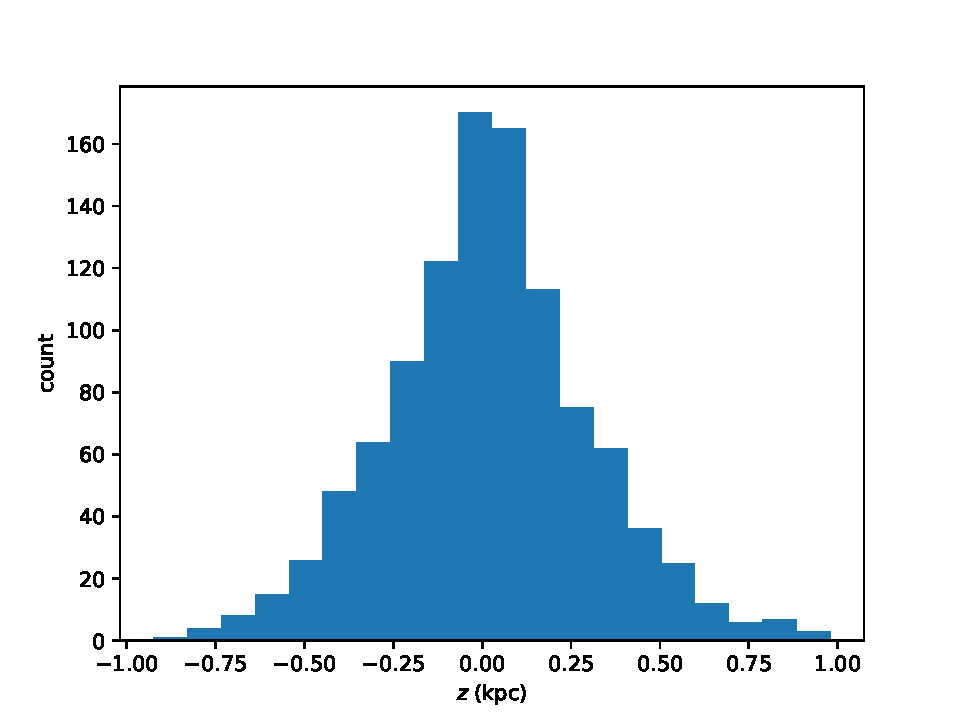
\includegraphics[width=4.5cm]{fig/dist_z.pdf}
\end{tabular}
    \caption{1000個の星の模擬データの1次元頻度分布}
    \label{distMockData}
\end{figure*}

\begin{table}
\begin{center}
%\scalebox{0.5}
%\scriptsize
%\footnotesize
%\small
\begin{tabular}{c|c|c|c} \hline
 \rowcolor{LightCyan}
 星の年齢 $\tau\ \mathrm{(Gyr)}$ & $\sigma_R\ \mathrm{(km\ s^{-1})}$ & $\sigma_{\phi}\ \mathrm{(km\ s^{-1})}$ & $\sigma_{z}\ \mathrm{(km\ s^{-1})}$\\
 \hline
 1.4 & 21.7 & 12.0 & 8.6\\
 \hline
 1.9 & 21.4 & 16.7 & 10.1\\
 \hline
 2.4 & 27.8 & 18.9 & 10.5\\
 \hline
 2.8 & 32.7 & 18.4 & 11.0\\
 \hline
 3.3 & 31.3 & 16.8 & 11.9\\
 \hline
 3.8 & 30.1 & 16.9 & 11.7\\
 \hline
 4.3 & 34.7 & 17.8 & 12.6\\
 \hline
 4.9 & 36.8 & 21.2 & 16.8\\
 \hline
 5.6 & 39.3 & 22.1 & 17.7\\
 \hline
 6.4 & 42.5 & 23.0 & 18.3\\
 \hline
 7.2 & 43.8 & 24.2 & 23.3\\
 \hline
 8.5 & 51.8 & 25.8 & 23.3\\
 \hline
\end{tabular} \label{VelocityDispersion}
\vspace{3mm}
\caption{模擬データ生成で用いた年齢と速度分散の対応表\cite{YL18}。}
\end{center}
\end{table}

%%%%%%%%%%%%%%%%%%%%%%%%%%%%%%%%%%%%%%%%%%%%%%%%%%%%%%%%%%%%%%%%%%%%%%%%%%%%%%%%
%%%%%%%%%%%%%%%%%%%%%%%%%%%%%%%%%%%%%%%%%%%%%%%%%%%%%%%%%%%%%%%%%%%%%%%%%%%%%%%%
%%%%%%%%%%%%%%%%%%%%%%%%%%%%%%%%%%%%%%%%%%%%%%%%%%%%%%%%%%%%%%%%%%%%%%%%%%%%%%%%

\section{模擬データの解析結果}
模擬データの解析では7つのパターンで模擬データ生成や解析方法を変更してオールト解析における7つの効果を調べた。表\ref{table4}、\ref{table5}はそれぞれの解析で用いた模擬データの設定と仮定を示している。asymmetric driftについては解析に際して入れる必要がある場合のみ模擬データに入れている。また、太陽は円盤面上に位置していると仮定している。

\begin{table}
\begin{center}
%\scalebox{0.5}
%\scriptsize
%\footnotesize
%\small
\begin{tabular}{l|c} \hline
 \rowcolor{LightCyan}
 パラメータ & 値\\
 \hline
 $A$ & 18 $\mathrm{km\,s^{-1} kpc^{-1}}$\\
 \hline
 $B$ & -11 $\mathrm{km\,s^{-1} kpc^{-1}}$\\
 \hline
 $C$ & -2 $\mathrm{km\,s^{-1} kpc^{-1}}$\\
 \hline
 $K$ & -1 $\mathrm{km\,s^{-1} kpc^{-1}}$\\
 \hline
 $U_{\odot}$ & 9 $\mathrm{km\,s^{-1}}$\\
 \hline
 $V_{\odot}$ & 11 $\mathrm{km\,s^{-1}}$\\
 \hline
 $W_{\odot}$ & 7.5 $\mathrm{km\,s^{-1}}$\\
 \hline
 $R_0$ & 8.2 $\mathrm{kpc}$\\
 \hline
\end{tabular}
\vspace{3mm}
\caption{模擬データ生成で用いた各パラメータの設定値。}
\label{table4}
\end{center}
\end{table}



\begin{table}
\begin{center}
%\scalebox{0.5}
%\scriptsize
%\footnotesize
%\small
\begin{tabular}{l|c|c} \hline
 \rowcolor{LightCyan}
 解析名 & asymmetric drift & 試行回数 \\
 \hline
 解析1: Asymmetric driftの解析結果への影響 & 有 & 3\\
 \hline
 解析2: 視線速度の有無による解析結果への影響 & 無 & 10\\
 \hline
 解析3: 速度楕円体の傾きの解析結果への影響 & 無 & 10\\
 \hline
 解析4: 太陽からの距離の解析結果への影響 & 無 & 10\\
 \hline
 解析5: 円盤面からの距離の解析結果への影響 & 無 & 10\\
 \hline
 解析6: サンプル数の解析結果への影響 & 無 & 10\\
 \hline
 解析7: $R_0$の値の解析結果への影響 & 有 & 3\\
 \hline
\end{tabular}
\vspace{3mm}
\caption{それぞれの解析で用いた設定。asymmetric driftの有無は、模擬データにasymmetric driftを入れたか入れないかを示している。試行回数は、模擬データを同じ設定値で生成し解析したパターン数。これは、ランダム性を可能な限り解消するためにいくつかのパターンで同じ解析を行って、全パターンの平均値を解析結果として用いている。}
\label{table5}
\end{center}
\end{table}

%%%%%%%%%%%%%%%%%%%%%%%%%%%%%%%%%%%%%%%%%%%%%%%%%%%%%%%%%%%%%%%%%%%%%%%%%%%%%%%%%%%%%%%%%%%%%%%%
%%%%%%%%%%%%%%%%%%%%%%%%%%%%%%%%%%%%%%%%%%%%%%%%%%%%%%%%%%%%%%%%%%%%%%%%%%%%%%%%%%%%%%%%%%%%%%%%
%%%%%%%%%%%%%%%%%%%%%%%%%%%%%%%%%%%%%%%%%%%%%%%%%%%%%%%%%%%%%%%%%%%%%%%%%%%%%%%%%%%%%%%%%%%%%%%%

\subsection{解析1: Asymmetric driftの解析結果への影響}
asymmetric driftの効果を入れた模擬データについて、asymmetric driftを考慮しない解析(観測方程式(\ref{ObsEq}))とasymmetric driftを考慮した解析(観測方程式(\ref{ObsEqAD}))との2通りの解析を行う。図(\ref{fig:Mock_AD})はその解析結果である。assyemtric drift無しと有りでは、$A,B,V_{\odot}$で明らかな違いがある。特に$V_{\odot}$ではasymmetric drift有りの解析結果の設定値との差が顕著であり、相対誤差

\begin{figure*}[htbp]
	\centering
	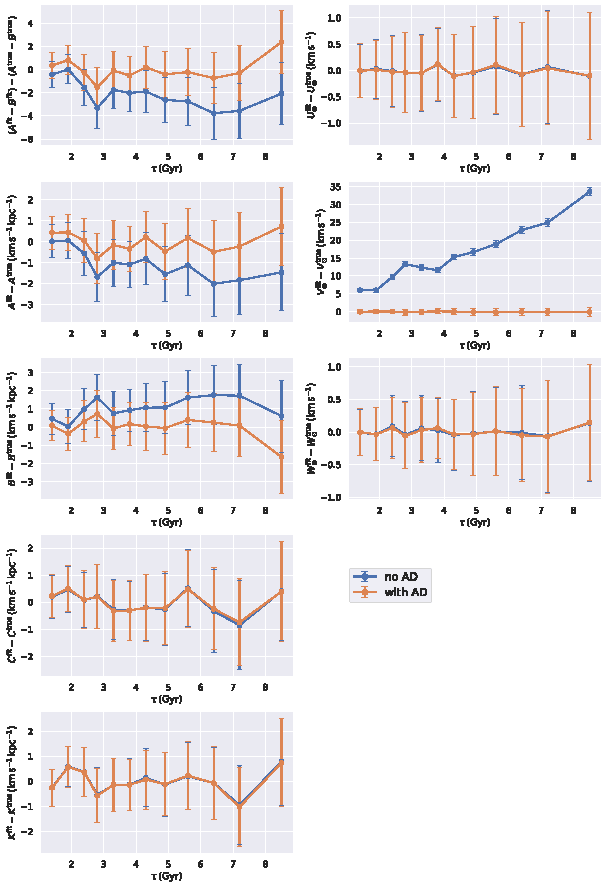
\includegraphics[width=15cm]{fig/Mock_AD.pdf}
	\caption{1000個の星の模擬データをasymmetric drift有り、無しで解析した結果。左図は各パラメータの解析結果。縦軸は各パラメータの値、横軸は模擬データに入れた速度分散に対応する年齢。trueは設定値、no ADはasymmetric driftを考慮していない解析結果、with ADはasymmetric driftを考慮した解析結果であることを示している。右図は左図の結果の絶対誤差と相対誤差、相対誤差のlogスケール。} \label{fig:Mock_AD}
\end{figure*}

%%%%%%%%%%%%%%%%%%%%%%%%%%%%%%%%%%%%%%%%%%%%%%%%%%%%%%%%%%%%%%%%%%%%%%%%%%%%%%%%%%%%%%%%%%%%%%%%
%%%%%%%%%%%%%%%%%%%%%%%%%%%%%%%%%%%%%%%%%%%%%%%%%%%%%%%%%%%%%%%%%%%%%%%%%%%%%%%%%%%%%%%%%%%%%%%%
%%%%%%%%%%%%%%%%%%%%%%%%%%%%%%%%%%%%%%%%%%%%%%%%%%%%%%%%%%%%%%%%%%%%%%%%%%%%%%%%%%%%%%%%%%%%%%%%

\subsection{解析2: 視線速度の有無による解析結果への影響}
視線速度を含めた観測方程式(\ref{ObsEq})での解析と含めない解析との結果を比較する(\ref{fig:Mock_vlos})。右側の図を見ると、$B$だけは速度分散無しの解析の方が有りの解析よりも少し良い精度となっているが、それ以外のパラメータでは視線速度有りの方が高い精度となっている。

\begin{figure*}[htbp]
	\centering
	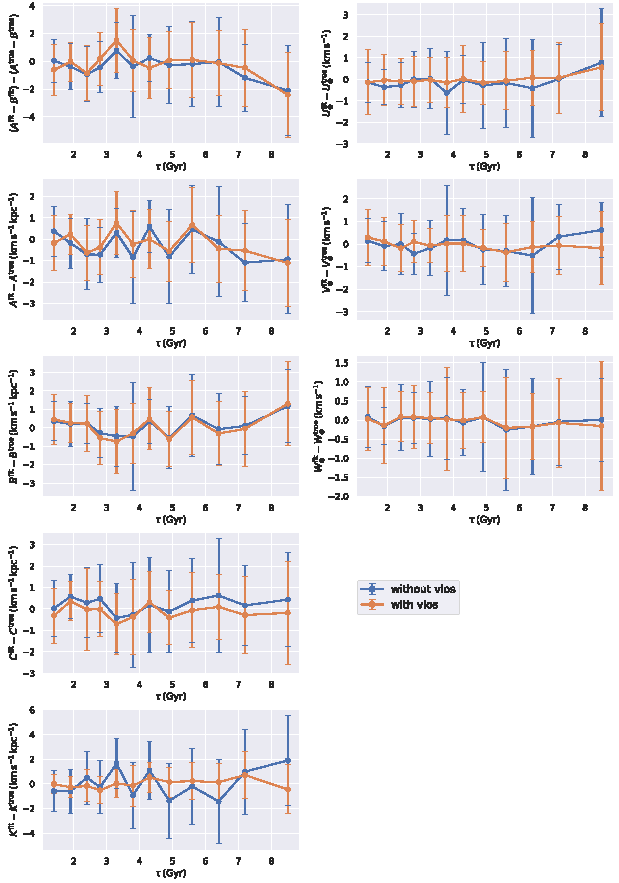
\includegraphics[width=15cm]{fig/Mock_vlos.pdf}
	\caption{視線速度の観測方程式有りと無しで解析したときの結果の絶対誤差、相対誤差と相対誤差のlogスケール。横軸は各パラメータとなっている。視線速度有りの解析の方が無しの解析よりも精度が高いことがわかる。右図は左図の結果の絶対誤差と相対誤差。} \label{fig:Mock_vlos}
\end{figure*}

%%%%%%%%%%%%%%%%%%%%%%%%%%%%%%%%%%%%%%%%%%%%%%%%%%%%%%%%%%%%%%%%%%%%%%%%%%%%%%%%%%%%%%%%%%%%%%%%
%%%%%%%%%%%%%%%%%%%%%%%%%%%%%%%%%%%%%%%%%%%%%%%%%%%%%%%%%%%%%%%%%%%%%%%%%%%%%%%%%%%%%%%%%%%%%%%%
%%%%%%%%%%%%%%%%%%%%%%%%%%%%%%%%%%%%%%%%%%%%%%%%%%%%%%%%%%%%%%%%%%%%%%%%%%%%%%%%%%%%%%%%%%%%%%%%

\subsection{解析3: 速度楕円体の傾きの解析結果への影響}
図\ref{fig:Mock_VE}は模擬データの速度$U$と$V$の間の速度楕円体の傾き$l_{UV}$を$0,10,20,30,40$度の5通りに設定した模擬データを生成し、それらをそれぞれ解析した結果である。この結果では$l_{UV}$の値による大きな違いは見られなかった。

\begin{figure*}[htbp]
	\centering
	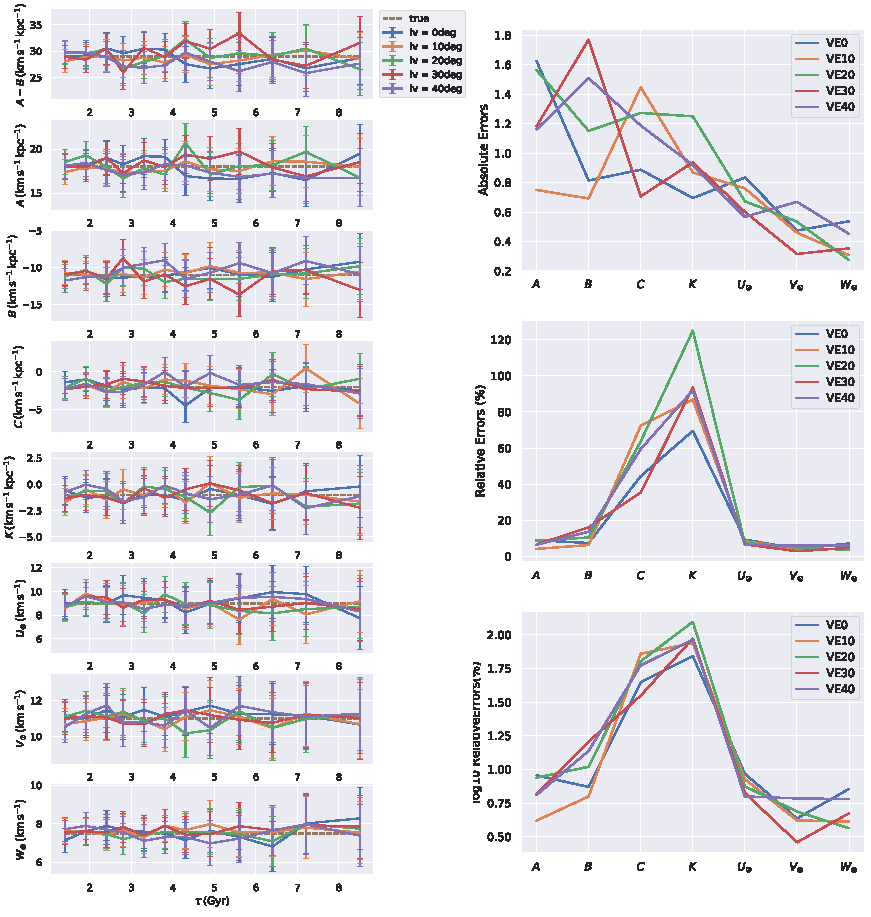
\includegraphics[width=15cm]{fig/Mock_VE.pdf}
	\caption{1000個の星の模擬データを速度楕円体の傾き$0,10,20,30,40$度で解析した結果。縦軸は各パラメータの値、横軸は模擬データに入れた速度分散に対応する年齢。} \label{fig:Mock_VE}
\end{figure*}


%%%%%%%%%%%%%%%%%%%%%%%%%%%%%%%%%%%%%%%%%%%%%%%%%%%%%%%%%%%%%%%%%%%%%%%%%%%%%%%%%%%%%%%%%%%%%%%%
%%%%%%%%%%%%%%%%%%%%%%%%%%%%%%%%%%%%%%%%%%%%%%%%%%%%%%%%%%%%%%%%%%%%%%%%%%%%%%%%%%%%%%%%%%%%%%%%
%%%%%%%%%%%%%%%%%%%%%%%%%%%%%%%%%%%%%%%%%%%%%%%%%%%%%%%%%%%%%%%%%%%%%%%%%%%%%%%%%%%%%%%%%%%%%%%%

\subsection{解析4: 太陽からの距離の解析結果への影響}
図\ref{fig:Mock_D}はサンプル星の太陽からの距離$D$の範囲を変えたときの解析結果である。$D<0.3\ \mathrm{kpc}$では他のパターンに比べて精度が悪い。
\begin{figure*}[htbp]
	\centering
	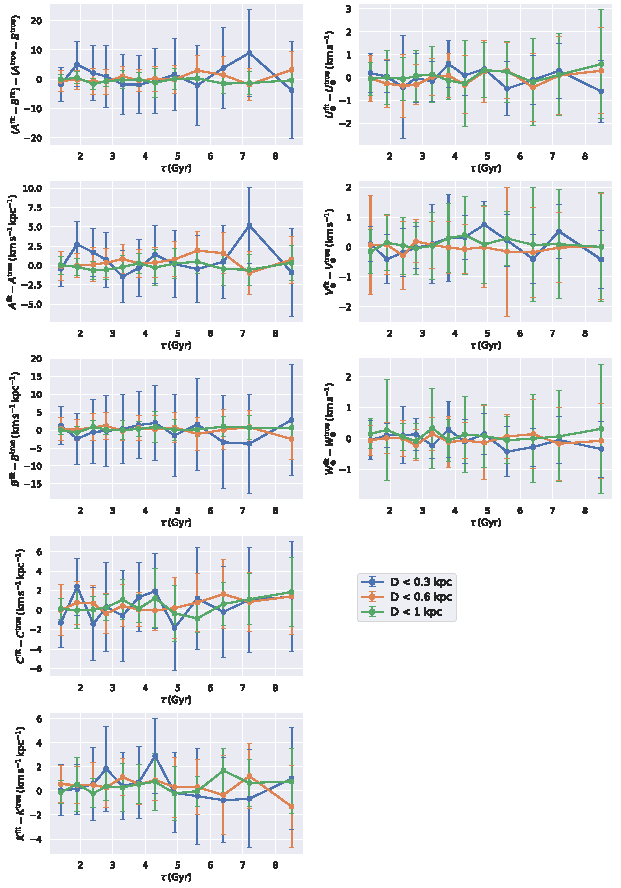
\includegraphics[width=15cm]{fig/Mock_D.pdf}
	\caption{1000個の星の模擬データを太陽からの距離を変えて$(D<0.3,0.4,,,1\  \mathrm{kpc})$解析した結果。縦軸は各パラメータの値、横軸は模擬データに入れた速度分散に対応する年齢。ラベルのD03は$D<0.3\ \mathrm{kpc}$、D04は$D<0.4\ \mathrm{kpc}$を意味する。} \label{fig:Mock_D}
\end{figure*}

%%%%%%%%%%%%%%%%%%%%%%%%%%%%%%%%%%%%%%%%%%%%%%%%%%%%%%%%%%%%%%%%%%%%%%%%%%%%%%%%%%%%%%%%%%%%%%%%
%%%%%%%%%%%%%%%%%%%%%%%%%%%%%%%%%%%%%%%%%%%%%%%%%%%%%%%%%%%%%%%%%%%%%%%%%%%%%%%%%%%%%%%%%%%%%%%%
%%%%%%%%%%%%%%%%%%%%%%%%%%%%%%%%%%%%%%%%%%%%%%%%%%%%%%%%%%%%%%%%%%%%%%%%%%%%%%%%%%%%%%%%%%%%%%%%

\subsection{解析5: 円盤面からの距離の解析結果への影響}
図\ref{fig:Mock_z}はサンプル星の円盤面からの距離$|z|$の範囲を変えて生成した模擬データの解析結果である。つまり、$|z|=100\ \mathrm{pc}$の場合、円盤面から$100\ \mathrm{pc}$以内の星を使用している。この解析結果からは$|z|$の値による大きな違いは見られなかった。

\begin{figure*}[htbp]
	\centering
	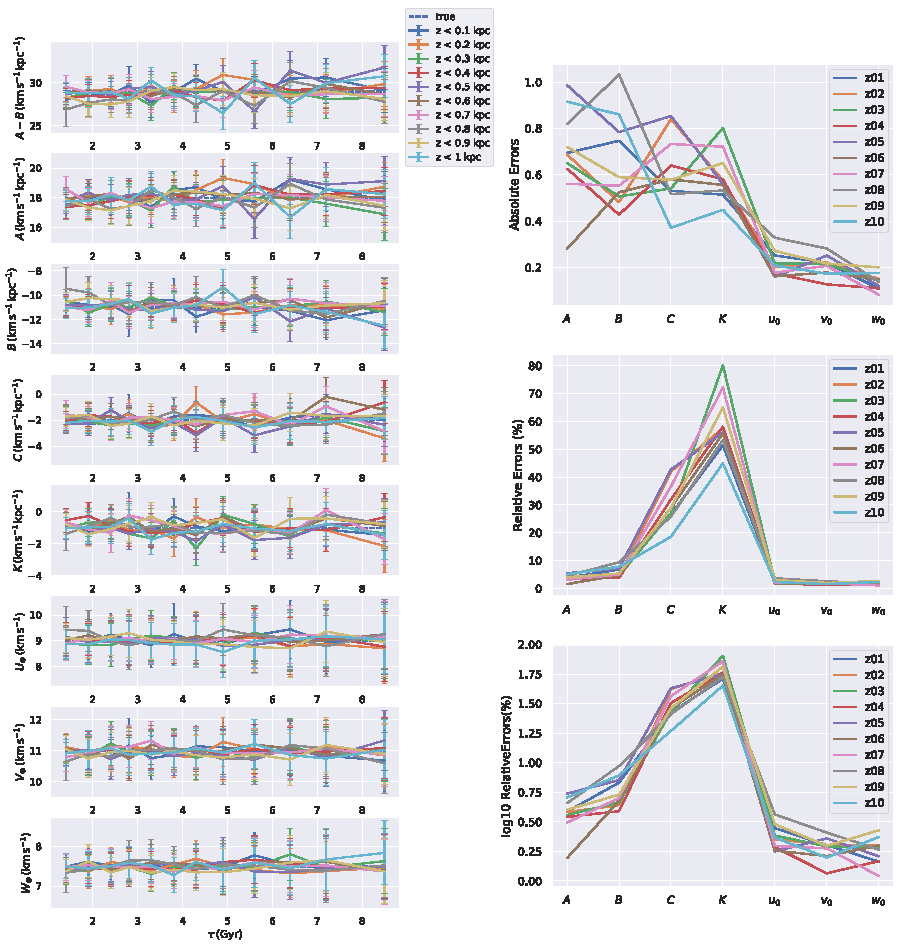
\includegraphics[width=15cm]{fig/Mock_z.pdf}
	\caption{1000個の星の模擬データを円盤面からの距離の範囲を変えて$(|z|<0.1,0.2,,,1 \mathrm{kpc})$解析した結果。縦軸は各パラメータの値、横軸は模擬データに入れた速度分散に対応する年齢。} \label{fig:Mock_z}
\end{figure*}

%%%%%%%%%%%%%%%%%%%%%%%%%%%%%%%%%%%%%%%%%%%%%%%%%%%%%%%%%%%%%%%%%%%%%%%%%%%%%%%%%%%%%%%%%%%%%%%%
%%%%%%%%%%%%%%%%%%%%%%%%%%%%%%%%%%%%%%%%%%%%%%%%%%%%%%%%%%%%%%%%%%%%%%%%%%%%%%%%%%%%%%%%%%%%%%%%
%%%%%%%%%%%%%%%%%%%%%%%%%%%%%%%%%%%%%%%%%%%%%%%%%%%%%%%%%%%%%%%%%%%%%%%%%%%%%%%%%%%%%%%%%%%%%%%%

\subsection{解析6: サンプル数の解析結果への影響}
\begin{figure*}[htbp]
	\centering
	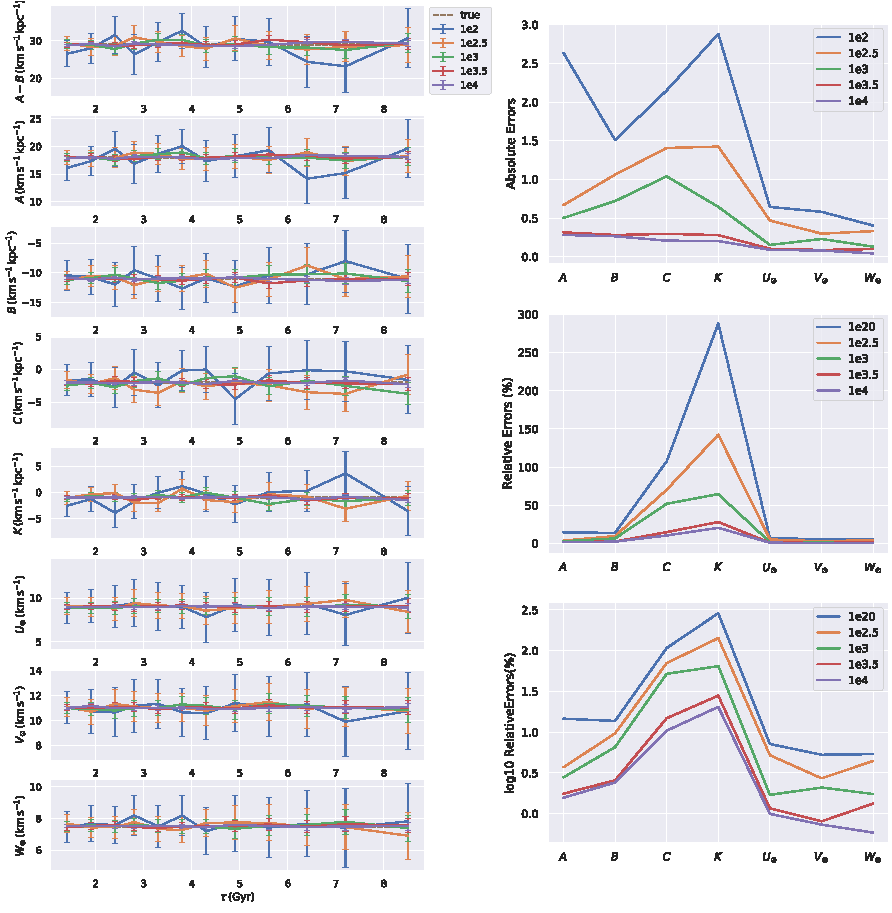
\includegraphics[width=15cm]{fig/Mock_N.pdf}
	\caption{サンプル数を変えて解析したときの結果の相対誤差。横軸は各パラメータ、縦軸は模擬データ生成時に設定した値と解析結果の値との相対誤差のlogスケール。サンプル数が多いほど相対誤差が小さくなっていることがわかる。} \label{fig:Mock_N}
\end{figure*}

%%%%%%%%%%%%%%%%%%%%%%%%%%%%%%%%%%%%%%%%%%%%%%%%%%%%%%%%%%%%%%%%%%%%%%%%%%%%%%%%%%%%%%%%%%%%%%%%
%%%%%%%%%%%%%%%%%%%%%%%%%%%%%%%%%%%%%%%%%%%%%%%%%%%%%%%%%%%%%%%%%%%%%%%%%%%%%%%%%%%%%%%%%%%%%%%%
%%%%%%%%%%%%%%%%%%%%%%%%%%%%%%%%%%%%%%%%%%%%%%%%%%%%%%%%%%%%%%%%%%%%%%%%%%%%%%%%%%%%%%%%%%%%%%%%

\subsection{解析7: $R_0$の値の解析結果への影響}
\begin{figure*}[htbp]
	\centering
	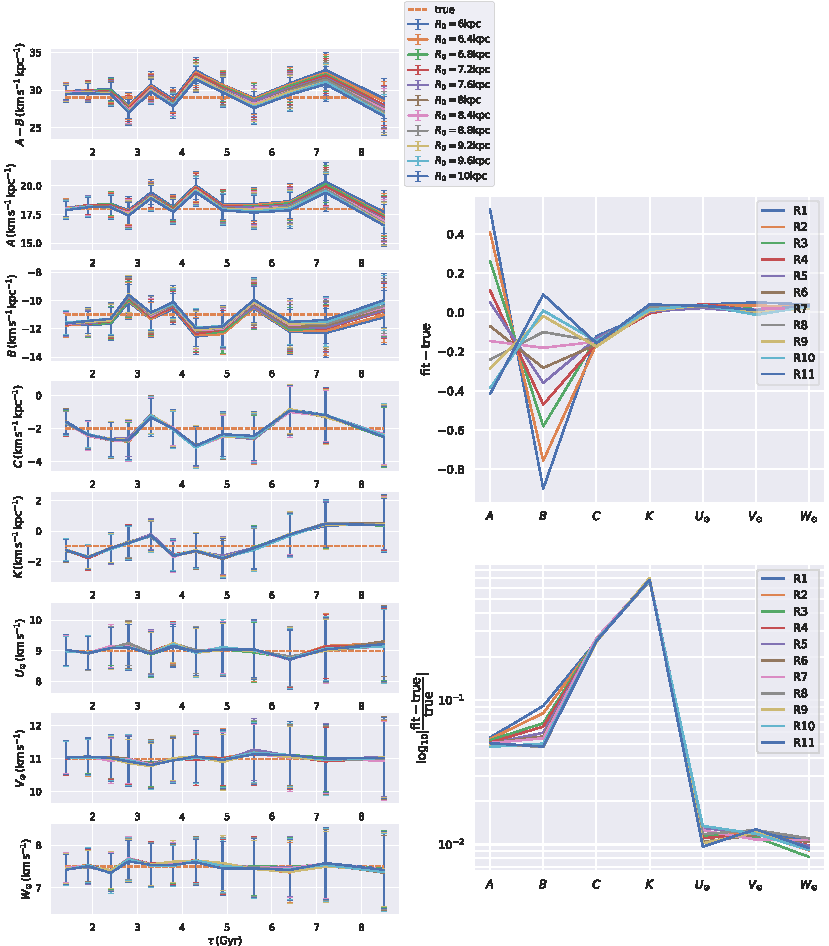
\includegraphics[width=15cm]{fig/Mock_R0.pdf}
	\caption{1000個の星の模擬データを太陽の銀河中心からの距離$R_0$を変えて$(R_0 = 6,6.4,6.8,,10 \mathrm{kpc})$解析した結果。縦軸は各パラメータの値、横軸は模擬データに入れた速度分散に対応する年齢。} \label{fig:Mock_R0}
\end{figure*}

\section{解析結果のまとめ}
全体的にオールト定数$C,K$の相対誤差が大きい結果となった。これは、これら2つのパラメータの絶対値がそれぞれ$2,1$と非常に小さいことが原因であると考えられる。また、顕著に見られる効果としてはasymmetric driftとサンプル数が大きい。サンプル数1000個の模擬データで$A,B,U_{\odot},V_{\odot},W_{\odot}$の相対誤差が10\%以下であることから、1000個のオーダーであれば銀河回転と太陽運動についてのパラメータについてはある程度の精度を確保できると考えられる。